% !TeX root = 00-main.tex
\documentclass[00-main.tex]{subfiles}

\begin{document}

\section{A Comparison of Integer- and Fractional-Order SEIR Models}

This section examines what is gained, both mathematically and empirically, by replacing an integer-order epidemic model with a fractional-order one.
The study in \cite{Is20} compares ordinary and Caputo fractional SEIR systems, derives both as mean-field descriptions of stochastic processes, and tests them against three measles epidemics from the pre-vaccination era.
It therefore provides a useful setting in which the choice of derivative can be examined without changing the underlying compartmental structure.
The discussion below retains the construction, comparison method, and principal results, while reporting only the conclusions of the lengthy equilibrium calculations.


\subsection{Integer- and fractional-order SEIR models}

Let $S(t)$, $E(t)$, $I(t)$, and $R(t)$ denote the proportions of susceptible, exposed, infectious, and recovered individuals, respectively, so that
\[
S(t)+E(t)+I(t)+R(t)=1.
\]
The initial conditions satisfy
\[
S(0),E(0),I(0),R(0)\geq0,
\qquad
S(0)+E(0)+I(0)+R(0)=1.
\]
Because the state variables are population proportions rather than population counts, the mass-action incidence is written as $\beta SI$; no additional division by the total population $N$ is required.

The parameter $\mu$ is the per-capita birth and natural death rate, $\beta$ is the transmission rate, $\delta$ is the rate at which exposed individuals become infectious, and $\sigma$ is the recovery rate.
Recruitment balances natural mortality because the population is assumed constant.
Infection transfers individuals from $S$ to $E$ at rate $\beta SI$, while $\delta^{-1}$ and $\sigma^{-1}$ describe the mean latent and infectious time scales in the classical formulation.
The resulting compartmental structure is displayed in Figure~\ref{fig:ch3-seir-flow}.

\begin{figure}[H]
\centering
\begin{tikzpicture}[
  node distance=2.3cm,
  compartment/.style={circle,draw,thick,minimum size=10mm,fill=blue!7},
  flow/.style={-{Stealth[length=2mm]},thick},
  loss/.style={-{Stealth[length=1.8mm]},thin},
  every edge quotes/.style={font=\scriptsize,inner sep=1pt}
]
\node[compartment] (S) {$S$};
\node[compartment,right=of S] (E) {$E$};
\node[compartment,right=of E] (I) {$I$};
\node[compartment,right=of I] (R) {$R$};
\coordinate[left=1.0cm of S] (birth);

\draw[flow] (birth) -- node[above,font=\scriptsize] {$\mu$} (S.west);
\draw[flow] (S) -- node[above,font=\scriptsize] {$\beta SI$} (E);
\draw[flow] (E) -- node[above,font=\scriptsize] {$\delta E$} (I);
\draw[flow] (I) -- node[above,font=\scriptsize] {$\sigma I$} (R);
\foreach \x in {S,E,I,R}{
  \draw[loss] (\x.south) -- ++(0,-0.75) node[below,font=\scriptsize] {$\mu \x$};
}
\end{tikzpicture}
\caption{Compartmental structure of the normalized SEIR model.}
\label{fig:ch3-seir-flow}
\end{figure}

The deterministic model is
\begin{equation}
\label{eq:ch3-classical-seir}
\left\{
\begin{aligned}
\frac{dS}{dt} &= \mu-\beta SI-\mu S,\\[3pt]
\frac{dE}{dt} &= \beta SI-(\mu+\delta)E,\\[3pt]
\frac{dI}{dt} &= \delta E-(\mu+\sigma)I,\\[3pt]
\frac{dR}{dt} &= \sigma I-\mu R.
\end{aligned}
\right.
\end{equation}
All four parameters in \eqref{eq:ch3-classical-seir} have units of inverse time.
The last equation is redundant once $R=1-(S+E+I)$ is imposed, but it is retained to display the complete SEIR flow.
The transmission coefficient $\beta$ is treated as a constant in this formulation.
Thus, although measles epidemics may exhibit seasonal transmission, seasonality is not represented through a time-dependent coefficient $\beta(t)$ in the model considered here.
This restriction keeps the compartmental structure fixed and allows the comparison to focus on the choice between integer- and fractional-order temporal operators.

The fractional formulation uses Caputo derivatives of a common order $0<\alpha\leq1$.
The same value of $\alpha$ is used in all four equations, so this is a commensurate fractional-order system rather than a model with a separate derivative order for each compartment.
Because ${}_{0}^{C}\!D_t^{\alpha}$ has dimension $\mathrm{time}^{-\alpha}$, every term on the right-hand side of the fractional system must have the same dimension.
Consequently, the coefficients obtained directly from the fractional stochastic process, denoted generically by $q$, have dimension
\[
[q]=\mathrm{time}^{-\alpha}.
\]
Such a coefficient cannot be interpreted immediately as an ordinary epidemiological rate, whose conventional dimension is $\mathrm{time}^{-1}$.
To retain that familiar interpretation, the paper introduces a new parameter $q_*$ satisfying
\[
q=q_*^{\alpha},
\qquad
[q_*]=\mathrm{time}^{-1}.
\]
It follows that $[q_*^{\alpha}]=\mathrm{time}^{-\alpha}$, as required by the fractional equation.
The subscript $*$ is only a label for this reparameterized rate; it does not denote multiplication, an optimal value, or an estimated value.
Applying this convention to the four epidemic rates gives $\mu_*^{\alpha}$, $\beta_*^{\alpha}$, $\delta_*^{\alpha}$, and $\sigma_*^{\alpha}$.
\begin{equation}
\label{eq:ch3-fractional-seir}
\left\{
\begin{aligned}
{}_{0}^{C}\!D_t^{\alpha}S &= \mu_*^{\alpha}-\beta_*^{\alpha}SI-\mu_*^{\alpha}S,\\[3pt]
{}_{0}^{C}\!D_t^{\alpha}E &= \beta_*^{\alpha}SI-(\mu_*^{\alpha}+\delta_*^{\alpha})E,\\[3pt]
{}_{0}^{C}\!D_t^{\alpha}I &= \delta_*^{\alpha}E-(\mu_*^{\alpha}+\sigma_*^{\alpha})I,\\[3pt]
{}_{0}^{C}\!D_t^{\alpha}R &= \sigma_*^{\alpha}I-\mu_*^{\alpha}R.
\end{aligned}
\right.
\end{equation}
When $\alpha=1$, one has $q=q_*$.
At the same time, the Caputo derivative becomes the ordinary first derivative, so both the equations and their rate dimensions reduce to those of the classical model.
Hence the comparison is nested, with the classical system appearing as a special case.
For $0<\alpha<1$, however, the fitted starred parameters should not be identified directly with the fitted rates of the classical ODE.
They belong to different parameterizations and coincide in the above reduction only when $\alpha=1$.

Directly comparing \eqref{eq:ch3-classical-seir} and \eqref{eq:ch3-fractional-seir} changes two features simultaneously: the differentiation operator and the parameter values.
To isolate these effects, an auxiliary $\alpha$-dependent ODE is introduced:
\begin{equation}
\label{eq:ch3-alpha-ode}
\left\{
\begin{aligned}
\frac{dS}{dt} &= \mu_*^{\alpha}-\beta_*^{\alpha}SI-\mu_*^{\alpha}S,\\[3pt]
\frac{dE}{dt} &= \beta_*^{\alpha}SI-(\mu_*^{\alpha}+\delta_*^{\alpha})E,\\[3pt]
\frac{dI}{dt} &= \delta_*^{\alpha}E-(\mu_*^{\alpha}+\sigma_*^{\alpha})I,\\[3pt]
\frac{dR}{dt} &= \sigma_*^{\alpha}I-\mu_*^{\alpha}R.
\end{aligned}
\right.
\end{equation}
Here the fitted value of $\alpha$ from the FDE is inserted into the coefficients, while the left-hand side remains integer order.
This system is a comparison device rather than a new mechanistic model: comparing it with the FDE holds the coefficients fixed and reveals the effect of the fractional clock itself.
There is also a dimensional caveat.
The ordinary derivative on the left-hand side has dimension $\mathrm{time}^{-1}$, whereas the inherited coefficients $q_*^{\alpha}$ have dimension $\mathrm{time}^{-\alpha}$.
Therefore, the auxiliary system should be understood only as the numerical analogue introduced in the original comparison, not as a separate dimensionally self-contained epidemiological model.


\subsection{Stochastic interpretation of the fractional model}

A common criticism of fractional epidemic models is that an ordinary derivative may simply be replaced by a fractional derivative without identifying a mechanism that produces it.
The construction in \cite{Is20} instead defines a family of stochastic SEIR processes indexed by the order $0<\alpha\leq1$.
Let
\[
\boldsymbol{X}^{(\alpha)}(t)
=\bigl(X_1^{(\alpha)}(t),X_2^{(\alpha)}(t),X_3^{(\alpha)}(t),X_4^{(\alpha)}(t)\bigr)
\]
denote the numbers of susceptible, exposed, infectious, and recovered individuals at time $t$.
The superscript $(\alpha)$ records the order of the stochastic process, and
\[
X_1^{(\alpha)}+X_2^{(\alpha)}+X_3^{(\alpha)}+X_4^{(\alpha)}=N.
\]
Unlike the deterministic variables in the preceding subsection, these variables are integer-valued random counts.
The paper takes $N$ as the population size and includes recruitment at rate $\mu N$ together with natural mortality in every compartment.
These demographic flows balance at the population level used to derive the normalized deterministic system; the transition table itself lists recruitment and deaths as separate stochastic changes.

The classical process is obtained by setting $\alpha=1$ and is denoted by $\boldsymbol{X}^{(1)}(t)$; this special case is a continuous-time Markov chain (CTMC).
Its state may change at any continuous time, but each change is one of a specified collection of events.
The Markov property means that, conditional on the present state, the distribution of the next event and its waiting time does not depend on the earlier history.
More precisely, if the possible transitions from a current state have rates $r_1,\ldots,r_m$, then the waiting time to the next event is exponentially distributed with total rate $r_1+\cdots+r_m$, and event $j$ is selected with probability $r_j/(r_1+\cdots+r_m)$.
The possible componentwise transitions and their rates are listed in Table~\ref{tab:ch3-ctmc-transitions}.
The event-name column is included to make the epidemiological meaning of each row explicit.

\begin{table}[H]
\centering
\caption{Transitions and rates of the stochastic SEIR process \cite{Is20}.}
\label{tab:ch3-ctmc-transitions}
\begin{tabular}{lll}
\toprule
Event & Transition & Rate \\
\midrule
Recruitment & $X_1^{(\alpha)}\to X_1^{(\alpha)}+1$ & $\mu N$ \\[3pt]
Infection or death from $S$ & $X_1^{(\alpha)}\to X_1^{(\alpha)}-1$ & $\displaystyle \beta\frac{X_1^{(\alpha)}X_3^{(\alpha)}}{N}+\mu X_1^{(\alpha)}$ \\[6pt]
Infection & $X_2^{(\alpha)}\to X_2^{(\alpha)}+1$ & $\displaystyle \beta\frac{X_1^{(\alpha)}X_3^{(\alpha)}}{N}$ \\[6pt]
Progression or death from $E$ & $X_2^{(\alpha)}\to X_2^{(\alpha)}-1$ & $(\mu+\delta)X_2^{(\alpha)}$ \\[3pt]
Progression & $X_3^{(\alpha)}\to X_3^{(\alpha)}+1$ & $\delta X_2^{(\alpha)}$ \\[3pt]
Recovery or death from $I$ & $X_3^{(\alpha)}\to X_3^{(\alpha)}-1$ & $(\mu+\sigma)X_3^{(\alpha)}$ \\[3pt]
Recovery & $X_4^{(\alpha)}\to X_4^{(\alpha)}+1$ & $\sigma X_3^{(\alpha)}$ \\[3pt]
Death from $R$ & $X_4^{(\alpha)}\to X_4^{(\alpha)}-1$ & $\mu X_4^{(\alpha)}$ \\
\bottomrule
\end{tabular}
\end{table}

As in the original presentation, the table records increases and decreases of individual components separately.
Consequently, a decrease row may combine more than one mechanism: for example, $X_1^{(\alpha)}\to X_1^{(\alpha)}-1$ can result from either infection or natural death.
At the same time, a transfer event contributes to two componentwise changes: one infection decreases $X_1^{(\alpha)}$ and increases $X_2^{(\alpha)}$.
Thus, the rows reproduce the marginal transition format of the original table and should not be interpreted as eight mutually independent epidemiological events.

A transition rate is an instantaneous event intensity, not a fixed waiting time.
In the classical case $\alpha=1$, if the current infection rate is
\[
r_{\mathrm{inf}}=\beta\frac{X_1^{(1)}X_3^{(1)}}{N},
\]
then, over a sufficiently short interval of length $\Delta t$, the probability of one infection event is
\[
r_{\mathrm{inf}}\Delta t+o(\Delta t).
\]
Hence infection events become more frequent when either the susceptible or infectious population increases.
This short-time CTMC interpretation applies specifically to $\alpha=1$; for $0<\alpha<1$, the altered waiting-time structure is described through the fractional forward equation and random-time construction below.

These event rates also explain the deterministic equations.
For example, recruitment increases $X_1$, whereas infection and susceptible mortality decrease it.
Therefore, the equation for its expectation is
\begin{equation}
\label{eq:ch3-expected-susceptible}
\frac{d}{dt}\mathbb{E}[X_1^{(1)}]
=\mu N-\frac{\beta}{N}\mathbb{E}[X_1^{(1)}X_3^{(1)}]
-\mu\mathbb{E}[X_1^{(1)}].
\end{equation}
This equation is not closed in the first moments because it contains the mixed second moment $\mathbb{E}[X_1^{(1)}X_3^{(1)}]$.
Under the mean-field approximation
\[
\mathbb{E}[X_1^{(1)}X_3^{(1)}]
\approx
\mathbb{E}[X_1^{(1)}]\mathbb{E}[X_3^{(1)}],
\]
the covariance between susceptible and infectious counts is neglected, since
\[
\mathbb{E}[X_1^{(1)}X_3^{(1)}]
=\mathbb{E}[X_1^{(1)}]\mathbb{E}[X_3^{(1)}]
+\operatorname{Cov}(X_1^{(1)},X_3^{(1)}).
\]
After applying this closure and dividing Equation~\eqref{eq:ch3-expected-susceptible} by $N$, one obtains
\[
\frac{dS}{dt}=\mu-\beta SI-\mu S.
\]
Applying the same event-balance argument to the other compartments produces the classical deterministic SEIR system in \eqref{eq:ch3-classical-seir}.
Thus, the ODE can be interpreted as a mean-field approximation to the expected behavior of the CTMC.

The fractional construction retains the same epidemiological events but changes the stochastic clock governing their occurrence.
The memoryless CTMC is introduced as a baseline: the fractional construction retains its epidemiological transition structure but evaluates the classical process on a random operational clock.
In physical time, this time change modifies the exponential waiting-time structure and introduces non-Markovian temporal dependence.
Let $\boldsymbol{X}^{(\alpha)}(t)$ denote the resulting fractional stochastic process.
Its state probabilities satisfy a fractional forward Kolmogorov equation in which the ordinary time derivative is replaced by a Caputo derivative of order $\alpha$.
For $\alpha=1$, this is the ordinary forward equation of the CTMC.
For $0<\alpha<1$, the process generally loses the Markov property because its temporal evolution retains information about past waiting times.

The relationship between the two stochastic processes is expressed through random-time subordination:
\[
\boldsymbol{X}^{(\alpha)}(t)
\overset{d}{=}
\boldsymbol{X}^{(1)}\!\left(T_{2\alpha}(t)\right),
\]
where $T_{2\alpha}(t)$ is a random operational time and $\overset{d}{=}$ denotes equality in distribution.
Thus, the fractional process can be viewed as the classical CTMC observed on a randomized clock.
When $\alpha=1$ the construction returns the ordinary process, whereas $0<\alpha<1$ alters its waiting-time structure.

To obtain deterministic equations from the fractional process, the probability-generating function is differentiated to derive equations for the expected compartment sizes.
The normalized fractional means are defined by
\[
S^{(\alpha)}(t)=\frac{1}{N}\mathbb{E}\!\left[X_1^{(\alpha)}(t)\right],\qquad
E^{(\alpha)}(t)=\frac{1}{N}\mathbb{E}\!\left[X_2^{(\alpha)}(t)\right],\qquad
I^{(\alpha)}(t)=\frac{1}{N}\mathbb{E}\!\left[X_3^{(\alpha)}(t)\right].
\]
The moment equations are not closed because infection contains a product of susceptible and infectious counts.
Applying the mean-field closure
\[
\mathbb{E}\!\left[X_1^{(\alpha)}X_3^{(\alpha)}\right]
\approx
\mathbb{E}\!\left[X_1^{(\alpha)}\right]
\mathbb{E}\!\left[X_3^{(\alpha)}\right]
\]
closes the system and produces the deterministic Caputo equations in \eqref{eq:ch3-fractional-seir}.
The FDE is therefore an approximation to the means of the fractional stochastic process, just as the classical ODE approximates the mean behavior of the CTMC.

The resulting chain of ideas is therefore
\[
\begin{aligned}
\text{CTMC transition rules}
&\longrightarrow \text{fractional stochastic clock}\\[3pt]
&\longrightarrow \text{fractional moment equations}\\[3pt]
&\longrightarrow \text{mean-field Caputo SEIR model}.
\end{aligned}
\]
This derivation does not imply that randomness has disappeared from the underlying epidemic.
Rather, it explains the deterministic fractional system as a population-level approximation and gives the fractional derivative a probabilistic origin.
The full fractional Kolmogorov equation and generating-function calculation are omitted here, but the transition table, randomized clock, and mean-field closure provide the essential connection.


\subsection{Dynamical and empirical comparison}

The analytical results provide the long-term baseline for the comparison.
The biologically feasible simplex is positively invariant, and the integer- and fractional-order systems have the same disease-free and endemic equilibria and the same threshold condition.
In particular, the disease-free equilibrium is locally asymptotically stable when $R_0<1$, whereas the endemic equilibrium is locally asymptotically stable when $R_0>1$.
The detailed Jacobian and Routh--Hurwitz calculations are not repeated here because the main distinction between the models lies in their transient behavior rather than their asymptotic states.

The numerical procedure solves the FDE using the deterministic time-subordination algorithm introduced in \cite{Is20}, while the ODE systems are solved by a Runge--Kutta method.
Figure~\ref{fig:ch3-original-fig2} first compares the classical ODE directly with fractional solutions obtained for several values of $\alpha$.
The FDE solution approaches the classical ODE solution as $\alpha\to1$.
For the parameters used in this simulation, decreasing $\alpha$ delays and raises the epidemic peak, while the original study describes the resulting outbreak duration as shorter.
These trends are specific to the model and parameterization used in the simulation and should not be treated as universal properties of all fractional epidemic models.

\begin{figure}[H]
\centering
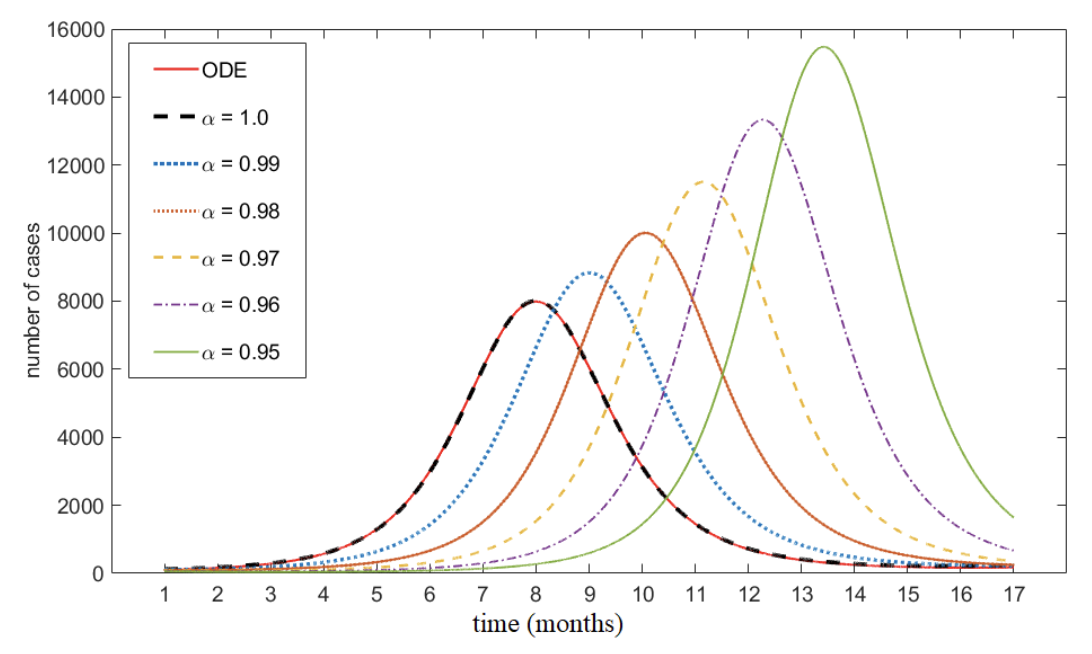
\includegraphics[width=0.88\textwidth]{img/Is20-fig2.png}
\caption{Effect of the fractional order on the simulated measles epidemic \cite{Is20}.}
\label{fig:ch3-original-fig2}
\end{figure}

The direct comparison in Figure~\ref{fig:ch3-original-fig2} changes both the derivative order and the associated parameterization.
To isolate the influence of the temporal operator more clearly, Figure~\ref{fig:ch3-original-fig3} compares the FDE with the auxiliary $\alpha$-dependent ODE in \eqref{eq:ch3-alpha-ode} while holding the $\alpha$-dependent coefficients fixed.
The two systems produce comparable numbers and amplitudes of transient peaks, but their peak times differ.
The FDE oscillations are stretched over a longer time scale and exhibit longer inter-epidemic periods, although both systems approach the same equilibrium.

\begin{figure}[H]
\centering
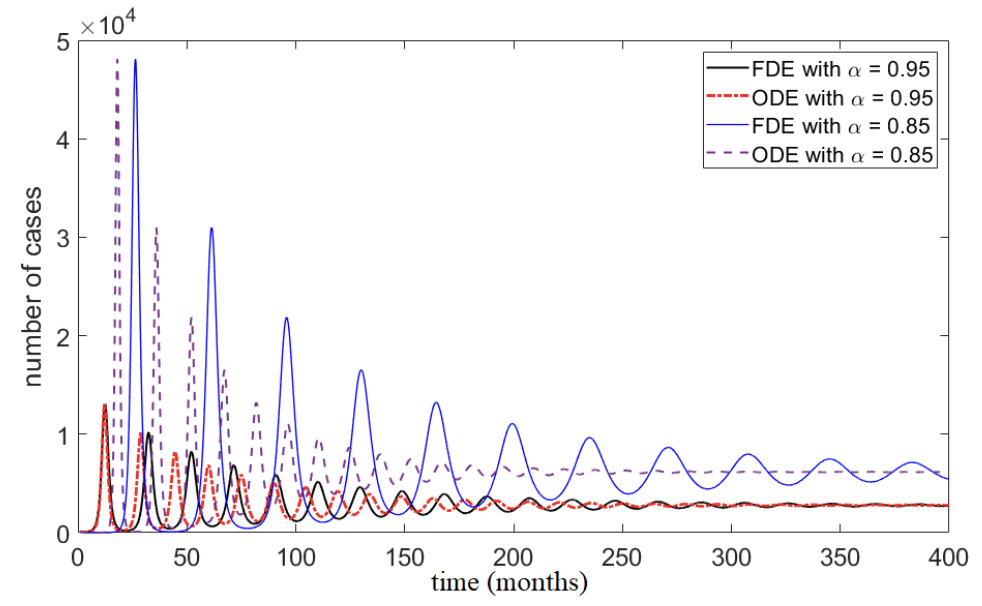
\includegraphics[width=0.88\textwidth]{img/Is20-fig3.png}
\caption{Comparison of the FDE and the corresponding $\alpha$-dependent ODE \cite{Is20}.}
\label{fig:ch3-original-fig3}
\end{figure}

Figure~\ref{fig:ch3-original-fig4} addresses a different question from Figure~\ref{fig:ch3-original-fig3}.
Rather than comparing the timing of full epidemic trajectories, it examines the linearized behavior near the endemic equilibrium.
As $\alpha$ decreases from one, the ordinary damped oscillations associated with conjugate complex eigenvalues are increasingly suppressed, and the corresponding phase-plane trajectories become less oscillatory.
Thus, the longer inter-epidemic timing observed in Figure~\ref{fig:ch3-original-fig3} should not be confused with preservation of the classical ODE oscillation pattern near equilibrium.

\begin{figure}[H]
\centering
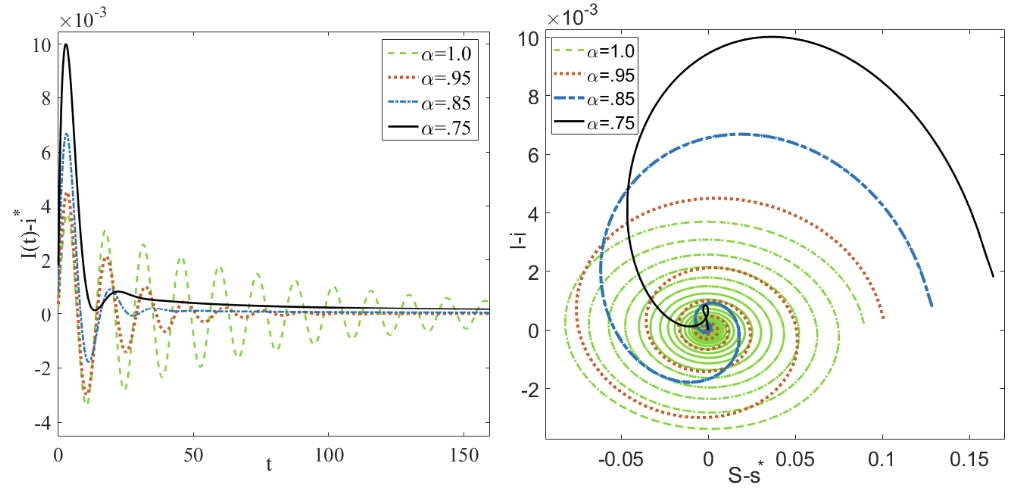
\includegraphics[width=0.92\textwidth]{img/Is20-fig4.png}
\caption{Suppression of damped oscillations near the endemic equilibrium as the fractional order decreases \cite{Is20}.}
\label{fig:ch3-original-fig4}
\end{figure}

The empirical comparison then asks whether these dynamical differences improve agreement with observed measles outbreaks.
Both models are fitted by ordinary least squares, using MATLAB's MultiStart and \texttt{fmincon} routines to minimize the squared difference between reported and simulated infectious cases.
Because the FDE contains the additional parameter $\alpha$, the study reports not only the sum of squared errors (SSE), but also the Akaike information criterion (AIC) and Bayesian information criterion (BIC), which penalize additional model complexity.

The data consist of monthly reports from New York and biweekly reports from London and Portsmouth during the pre-vaccination era.
The estimated fractional orders are
\[
\widehat{\alpha}_{\mathrm{New\ York}}=0.999999999524,
\qquad
\widehat{\alpha}_{\mathrm{London}}=0.999999999614,
\qquad
\widehat{\alpha}_{\mathrm{Portsmouth}}=0.875784505546.
\]
For New York and London, the estimates differ from one only at approximately the ninth decimal place, so the fitted FDEs are effectively indistinguishable from the fitted ODEs.
For Portsmouth, the estimated order is appreciably below one and the FDE gives a slightly better fit.
Nevertheless, the SSE, AIC, and BIC values remain similar across the two formulations for all three data sets.

\begin{figure}[H]
\centering
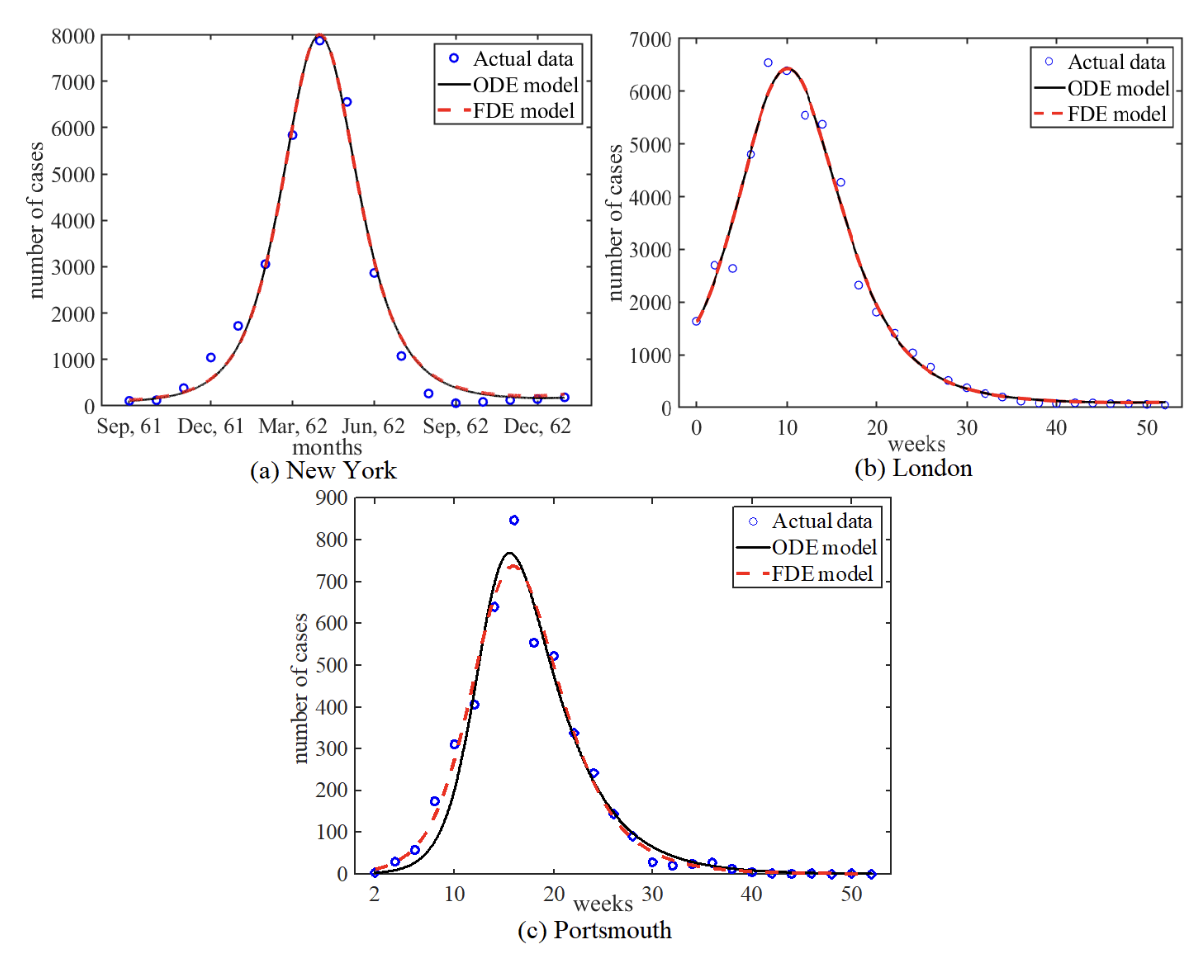
\includegraphics[width=0.88\textwidth]{img/Is20-fig5.png}
\caption{Comparison of integer- and fractional-order fits to three pre-vaccination measles epidemics \cite{Is20}.}
\label{fig:ch3-original-fig5}
\end{figure}

Figure~\ref{fig:ch3-original-fig5} summarizes the central empirical result.
The additional fractional order does not automatically improve the model.
In two of the three data sets, estimation effectively recovers the classical case by returning $\alpha\approx1$.
Only the Portsmouth data favor an order clearly below one, and even there the improvement is modest rather than decisive.


\subsection{Assessment of fractionalization}

The comparison leads to a qualified view of fractionalization whose value should be assessed at three distinct levels.
At the mathematical level, the additional order $\alpha$ provides flexibility in epidemic-peak timing, transient oscillations, and inter-epidemic periods.
At the mechanistic level, the stochastic construction relates the Caputo system to a classical stochastic SEIR process evaluated on a random operational clock, so the fractional derivative is not introduced solely as a formal replacement.
At the empirical level, however, this additional structure is useful only if it improves agreement with observations or prediction of epidemiologically relevant quantities.
These three forms of value should not be conflated: a mathematically well-motivated model need not provide a better empirical description, and a better fit alone does not verify the proposed stochastic mechanism.

The three measles data sets provide deliberately limited evidence in favor of the FDE.
For New York and London, the estimated orders differ from one only at approximately the ninth decimal place, so the FDE and ODE are equivalent up to possible numerical round-off effects.
For Portsmouth, the estimate is approximately $0.88$ and the FDE performs better, but the improvement in SSE, AIC, and BIC is modest.
The study therefore shows that a fractional model may either reduce numerically to its classical counterpart or offer additional flexibility, depending on the data set; it does not establish a general superiority of FDEs over ODEs.

An estimated value $\widehat{\alpha}<1$ also requires careful interpretation.
It indicates that the fitted fractional model captures temporal behavior not represented by the selected classical model, but it is not by itself proof of a particular biological memory mechanism.
Similar discrepancies could arise from omitted seasonality, time-varying transmission, reporting errors, population heterogeneity, or other forms of model misspecification.
Consequently, the interpretation of $\alpha$ should be supported by the model construction, the data, and sensitivity analyses rather than inferred solely from its fitted numerical value.

A practical preference for the FDE should therefore require several forms of evidence.
The estimate of $\alpha$ should be meaningfully separated from one, and the improvement should remain after AIC or BIC penalizes the additional parameter.
The improvement should also occur in the epidemic feature relevant to the modeling objective, such as peak timing or inter-epidemic spacing, and should remain reasonably stable under changes in initial conditions, fitting intervals, and numerical schemes.
As a further methodological recommendation beyond the analysis performed in \cite{Is20}, out-of-sample predictive validation would provide stronger evidence than in-sample goodness of fit alone.

Parameter identifiability is equally important because changes in $\alpha$ may be compensated by changes in $\beta_*$, $\delta_*$, $\sigma_*$, or $\mu_*$, producing similar epidemic curves.
The near-unit estimates for New York and London may therefore be read not only as a return to the classical model, but also as an indication that those data do not require a distinct fractional order.
Determining whether $\alpha$ and the epidemiological rates can be estimated separately and reliably is necessary before assigning a strong interpretation to the fitted order.

These empirical and inferential demands must be weighed against computational cost.
Because the Caputo derivative is nonlocal, evaluating a solution at a new time generally requires information from its preceding history.
Repeatedly solving the FDE during parameter estimation is therefore more expensive than solving the corresponding ODE, and the additional order enlarges the optimization problem.
The original study consequently suggests that fractional modeling is most promising when sufficiently large and refined data sets are available together with reliable numerical algorithms.

The central question is therefore not merely whether an FDE can fit epidemic data, but whether its fractional order, rate parameters, mechanistic interpretation, and empirical improvement are sufficient to justify the extra structure.
These broader limitations and ambiguities are examined critically in the next chapter.

\ifSubfilesClassLoaded{\printbibliography}{}

\end{document}
